\section{Related Work}
This section explores the related work inside the RTI area and explains the
underlying principles. The project is currently only concerned with the viewing
part, so that will covered in most depth.

\subsection{RTI Theory and Workflows}

The RTI workflow is a three step one (see~\autoref{capture}) in our context
(with the hunt for the physical object excluded). The object is placed central under
some capturing device (like~\autoref{dome}). A camera is
statically mounted on top. And the lights are setup to be lit in
order to have a different light position for all captured images. From these
images the RTI coefficents are calculated (see~\autoref{overview1}).

\fig{capture}{RTI Workflow}{RTI workflow, courtesy of CHI\cite*{noauthor_cultural_nodate-1}.}
\fig{dome}{RTI Dome}{RTI dome, from Malzbender et al\cite*{malzbender_polynomial_2001}.}

\begin{figure}
\begin{subfloat}[]{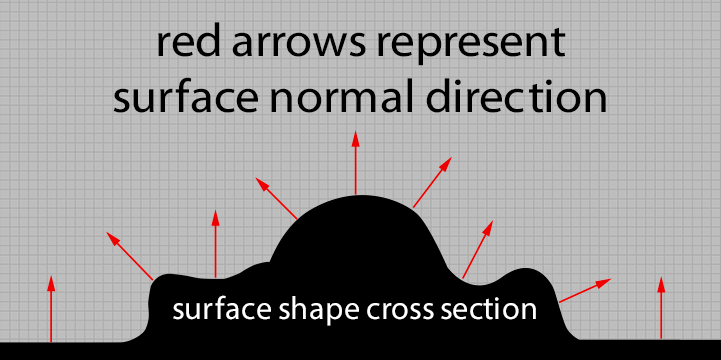
\includegraphics[max width=0.32\linewidth]{images/normals_01}}\end{subfloat}
\begin{subfloat}[]{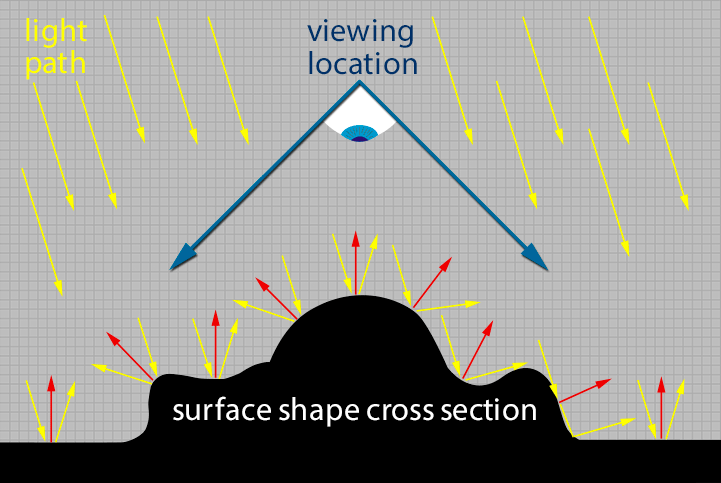
\includegraphics[max width=0.32\linewidth]{images/normals_02}}\end{subfloat}
\begin{subfloat}[]{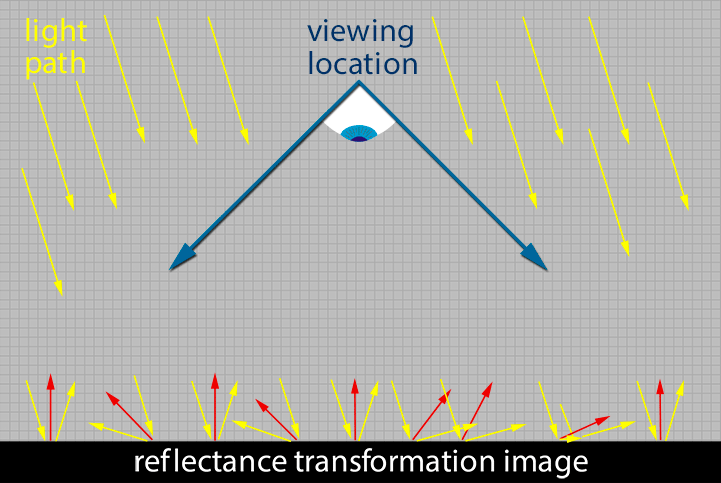
\includegraphics[max width=0.32\linewidth]{images/normals_03}}\end{subfloat}
\caption[RTI Overview]{\emph{a} shows the to be captured object's normals.
  \emph{b} shows the object with a single viewpoint and light source (in the
  capturing dome the eye would be camera). \emph{c} visualizes the RTI viewing
  process. Images from CHI\cite*{noauthor_cultural_nodate}.}
\label{overview1}
\end{figure}





\todoT{Workflow Comparisions}

\subsection{Fileformats}\label{sec_relfile}
The most comprehensive overview on the current state of the art is done by the
American library of congress as part of its Digital preservation effort, with
the sections on the ptm\cite{library_of_congress_polynomial_2018} and
rti\cite{library_of_congress_reflectance_2018} formats. The current PTM
specification by Malzbender and Gelb\cite{malzbender_polynomial_nodate}.
\todoT{File formats comparison}
\todoD{Size tables/graphes of ptm/rti/btf(.zip)}
\todoT{Streaming architectures}

\subsection{RTI Viewers}
\todoT{Viewer Comparision}
\todoT{No extensible architecture}
\todoT{No real open source (email before or one file sources)}

